%%%%%%%%%%%%%%%%%%%%%%%%%%%%%%%%%%%%%%%%%%%%%%%%%%%%%%%%%%%%%%%%%%%%%%%%%%%%%%%%%%%%%
% 			Facultad de Ciencias, UAEM.							Agosto de 2014
% 
%	Alumno: 				Emanuel García Pérez
%	Asginatura:				Catedra de Ciencias
%	Proyecto:				Presentación - Artículo
%	Tema:					"Desarrollo de un Sistema de Recuperación de Información
%							para Documentos Científicos del Área de Ciencias de la 
%   						Computación"
%
%%%%%%%%%%%%%%%%%%%%%%%%%%%%%%%%%%%%%%%%%%%%%%%%%%%%%%%%%%%%%%%%%%%%%%%%%%%%%%%%%%%%%


\documentclass{beamer}
 
%\usepackage[spanish,activeacute]{babel}
\usepackage[latin1]{inputenc}
\usepackage{beamerthemeshadow}
\usepackage{graphicx}

\title{\textbf{Desarrollo de un Sistema de Recuperaci\'on de Informaci\'on para Documentos Cient\'ificos del \'Area de Ciencias de la Computaci\'on}} 
\author{Emanuel Garc\'ia P\'erez}
\date{\today}

\begin{document}

\frame[allowframebreaks]{\titlepage}
\section[Contenidos]{}
\frame{
\transdissolve[duration=0.2]
\tableofcontents
} 

\section{CONCEPTOS \& DEFINICIONES}
\subsection{SRI para documentos cient\'ificos}
\frame{
\transdissolve[duration=0.2]
\frametitle{Sistema de Recuperaci\'on de Informaci\'on (I)}
Un Sistema de Recuperaci\'on de Informaci\'on(SRI) es un proceso que posee capacidad para recuperar, almacenar y mantener informaci\'on para distintos fines, seg\'un el contexto de su aplicaci\'on.\\
Existen diversas propuestas sobre la organizaci\'on(estructura) interna de un SRI, se eligi\'o utilizar una que se basa en los siguientes elementos:
}

\frame{
\transdissolve[duration=0.2]
\frametitle{Sistema de Recuperaci\'on de Informaci\'on (II)}
\begin{itemize}
\item Documentos: Fuente de informaci\'on sobre la cual se pretende realizar b\'usquedas.
\item Consultas: Generadas por los usuarios del SRI que tienen por objetivo recuperar la informaci\'on a la cual el sistema provee acceso.
\item Representaci\'on de los Documentos: Consultas y las relaciones que se definan entre ellas que sean definidas teniendo en cuenta el \'ambito de aplicaci\'on del SRI.
\item Funci\'on de Evaluaci\'on: Determina la pertinencia de cada documento recuperado para dar soluci\'on a la consulta del usuario.
\end{itemize}
}

\frame{
\transdissolve[duration=0.2]
\frametitle{Sistema de Recuperaci\'on de Informaci\'on (III)}
Los principales tipos de SRI que actualmente operan en Internet son: directorios(Yahoo), buscadores(Google), y meta-buscadores(Ixquick). Podemos asegurar que existen implementaciones de SRI en Internet que utilizan diferentes m\'etodos de b\'usqueda sobre contextos generales o particulares, incluyendo implementaciones particulares para el incremento de la relevancia de los resultados a presentar al usuario.\\
Entre estos destacan los meta-buscadores, debido a que su modularidad permite que los componentes del SRI sean desarrollados para cubrir las necesidades establecidas para una implementaci\'on particular.
}

\frame{
\transdissolve[duration=0.2]
\frametitle{Sistema de Recuperaci\'on de Informaci\'on (IV)}
Para desarrollar el SRI particular requerido por el presente trabajo, se considerar\'on los siguientes componentes: 
\begin{enumerate}
\item El componente que captura la consulta de usuario y la expande, generando consultas similares para expandir el espectro de b\'usqueda.
\item El componente que accede a las fuentes de datos y recupera de cada una de ellas los documentos resultantes de la ejecuci\'on de una consulta.
\item El componente que aplica la funci\'on de evaluaci\'on a los documentos obtenidos de cada fuente para ordenar el listado final para el usuario.
\end{enumerate}
}


\frame{
\transdissolve[duration=0.2]
\frametitle{SRI para documentos cient\'ificos de Ciencias de la Computaci\'on (I)}
Hay diversas iniciativas para la generaci\'on de SRI de proposito especifico en \'areas particulares, pero no se encontr\'o evidencia de que existan implementaciones que sean aplicadas a bases de datos de documentos cient\'ificos de Ciencias de la Computaci\'on. \\
Tampoco se encontr\'o evidencia de productos que implementen soluciones complementarias para aspectos clave, como expansi\'on de consultas considerando el contexto de la b\'usqueda y la aplicaci\'on de m\'etodos de evaluaci\'on a los documentos en base a la calidad de los mismos.
}

\frame{
\transdissolve[duration=0.2]
\frametitle{SRI para documentos cient\'ificos de Ciencias de la Computaci\'on (II)}
Explotando las capacidades que poseen los meta-buscadores, se consider\'o factible generar un SRI que utilice bases de datos de otros buscadores que sean especificos para la recuperaci\'on de documentos cient\'ificos. Tambi\'en se opto por desarrollar componentes complementarios, tanto para el tratamiento de las consultas como para la aplicaci\'on de un algoritmo de ranking especifico para evaluar el tipo de resultados con el que se desea operar, seg\'un distintas m\'etricas ampliamente aceptadas por la comunidad cient\'ifica, asignando a cada documento una calificaci\'on que servir\'a de referencia para establecer el orden de los resultados de la consulta.
}

\subsection{Expansi\'on de la consultas en un SRI y ontolog\'ias}
\frame{
\transdissolve[duration=0.2]
\frametitle{Expansi\'on de consultas}
Un SRI posee varias alternativas para lograr optimizar el proceso de b\'usqueda de informaci\'on, una de ellas consiste en tomar la consulta del usuario y ampliarla a partir de agregar diversos t\'erminos, obtenidos com\'unmente a trav\'es de fuentes externas, manteniendo coherencia con el dominio de la consulta. Este m\'etodo es conocido como expansi\'on de consultas(QE); los t\'erminos adicionales generan nuevas consultas, denominadas expansiones. De esta forma el SRI puede acceder a una mayor cantidad de documentos relevantes para el usuario, obteniendo listados de resultados individuales por cada expansi\'on, los cuales posteriormente son unificados y ponderados antes de ser devueltos al usuario. 
}

\frame{
\transdissolve[duration=0.2]
\frametitle{Ontolog\'ia (I)}
Existen diferentes opciones para implementar un proceso de expansi\'on de consultas para un SRI, algunas son: tesauros, diccionarios, sistemas expertos, etc. Para el caso particular del SRI a generar se hace uso de una ontolog\'ia de dominio especifica para una sub\'area tem\'atica de las Ciencias de la Computaci\'on.\\
Una ontolog\'ia se define como una forma de representar el conocimiento de un \'ambito especifico, que utiliza los t\'erminos y relaciones que conforman su vocabulario base, agregando elementos que permiten extender el vocabulario, como relaciones entre conceptos, permitiendo organizarlos jerarqu\'icamente.
}
 
\frame{
\transdissolve[duration=0.2]
\frametitle{Ontolog\'ia (II)}
Adaptando la definici\'on anterior al \'area de Ciencias de la Computaci\'on, se puede considerar a una ontolog\'ia como un esquema conceptual correspondiente a un dominio acotado, que permite la comunicaci\'on y la transmisi\'on de informaci\'on entre sistemas. Esto constituye una herramienta de gran utilidad para la recuperaci\'on y an\'alisis del conocimiento a trav\'es de una estrcutura de clases y subclases que adquiere sentido con las relaciones, propiedades y reglas definidas entre las instancias de las mismas.
}

\subsection{M\'etricas para la evaluaci\'on de documentos cient\'ificos}
\frame{
\transdissolve[duration=0.2]
\frametitle{Caracter\'isticas evaluables}
Para desarrollar el m\'etodo particular para evaluar los documentos se opto por considerar las siguientes caracter\'isticas: 
\begin{enumerate}
\item La calidad de la fuente de publicaci\'on, refiri\'endose a d\'onde se ha publicado el art\'iculo, pudiendo ser una revista cient\'ifica o un congreso o reuni\'on cient\'ifica.
\item La calidad de los autores, valorando la importancia que hubieran tenido las publicaciones que hayan realizado a lo largo de su carrera.
\item La calidad del art\'iculo en si, considerando la antig\"uedad del mismo y la cantidad de veces que haya sido citado en otros documentos.
\end{enumerate}
}

\frame{
\transdissolve[duration=0.2]
\frametitle{M\'etricas de evaluaci\'on (I)}
Para cada una de las caracter\'isticas elegidas para valorar un art\'iculo se distinguen diversos indicadores bibliom\'etricos preexistentes que han sido validados por la comunidad cient\'ifica. A continuaci\'on se enuncian y explican aquellos que ser\'an utlizados para evaluar cada una de las caracter\'isticas establecidas.
}

\frame{
\transdissolve[duration=0.2]
\frametitle{M\'etricas de evaluaci\'on (II)}
\begin{itemize}
\item Calidad de la fuente de publicaci\'on
	\begin{enumerate}
	\item Publicaci\'on en revista cient\'ifica
		\begin{itemize}
		\item Factor de Impacto (IF)
		\item SCImago Journal Rank (SJR)
		\end{itemize}
	\item Publicaci\'on en Congreso o Evento Cient\'ifico
		\begin{itemize}
		\item Ranking CORE
		\end{itemize}
	\end{enumerate}
\item Calidad de los autores
	\begin{enumerate}
	\item \'Indice H
	\item \'Indice G
	\end{enumerate}
\item Calidad del art\'iculo
	\begin{enumerate}
	\item \'Indice AR
	\item Cantidad de citas 
	\end{enumerate}
\end{itemize}
}

\frame{
\transdissolve[duration=0.2]
\frametitle{Calidad de la fuente de publicaci\'on (I)}
\begin{itemize}
\item Publicaci\'on en revista cient\'ifica
	\begin{itemize}
	\item Factor de Impacto(IF) [Web of Knowledge] \\ Permite medir la importancia que ha tenido una revista a partir de las citas que han recibido los art\'iculos que se han publicado en ella en un a\~no en particular.
	\item SCImago Journal Rank(SJR) [Grupo SCImago(Scopus)] \\ Est\'a inspirado en el PageRank de Google para evaluar el impacto de una publicaci\'on de acuerdo al n\'umero de citas recibidas con respecto a la relevancia de las publicaciones que la citan. Este establece una clasificaci\'on de acuerdo a ciertos par\'ametros: \'area de conocimiento, categor\'ia, pa\'is, etc.
	\end{itemize}
\end{itemize}
}

\frame{
\transdissolve[duration=0.2]
\frametitle{Calidad de la fuente de publicaci\'on (II)}
\begin{itemize}
\item Publicaci\'on en Congreso o Evento Cient\'ifico
	\begin{itemize}
	\item Ranking CORE [Computer Research \& Education(Australia)] \\ Un congreso o conferencia es clasificado, seg\'un su importancia, en un determinado nivel preestablecido: A*, A, B y C, respectivamente.
	\end{itemize}
\end{itemize}
}

\frame{
\transdissolve[duration=0.2]
\frametitle{Calidad de los autores (I)}
\begin{itemize}
\item \'Indice H [Jorge E. Hirsch] \\ Sse calcula en base a la distribuci\'on de las citas que han recibido las publicaciones de un determinado autor. Para hallarlo, solo basta ordenar de forma descendente las publicaciones de un autor por el n\'umero de veces que ha sido citada cada publicaci\'on, un autor tiene \'indice h si el h de sus Np trabajos recibe al menos h citas cada uno, y los otros (Np - h) trabajos tienen como m\'aximo h citas cada uno.
\end{itemize}
}

\frame{
\transdissolve[duration=0.2]
\frametitle{Calidad de los autores (II)}
\begin{itemize}
\item \'Indice G [Leo Egghe] \\ Los art\'iculos de un autor son ordenados de manera descendente de acuerdo con el n\'umero de citas recibidas por cada uno de ellos, similar al \'Indice H. Aquel n\'umero mayor en el orden del ranking donde la sumatoria de citas recibidas por el autor sea mayor o igual al cuadrado del n\'umero de mayor orden, es considerado como el \'indice G.
\end{itemize}
}

\frame{
\transdissolve[duration=0.2]
\frametitle{Calidad del art\'iculo}
\begin{itemize}
\item \'Indice AR [Bihui Jin] \\ Permite evaluar la calidad de una colecci\'on de publicaciones, este indicador combina la cantidad de citas con la antig\"uedad de cada publicaci\'on, para as\'i establecer una valoraci\'on de la colecci\'on. Es un \'indice complementario del \'Indice H.
\item Cantidad de citas \\ La cantidad de citas recibidas, por s\'i solas, tambi\'en es utilizada como m\'etrica para evaluar la calidad de un documento cient\'ifico en particular.
\end{itemize}
}


\section{RECURSOS \& DISE\~NO}
\subsection{Estructura \& Funcionamiento del SRI}
\frame{
\transdissolve[duration=0.2]
\frametitle{SRI(meta-buscador)}
\begin{figure}
  \centering
    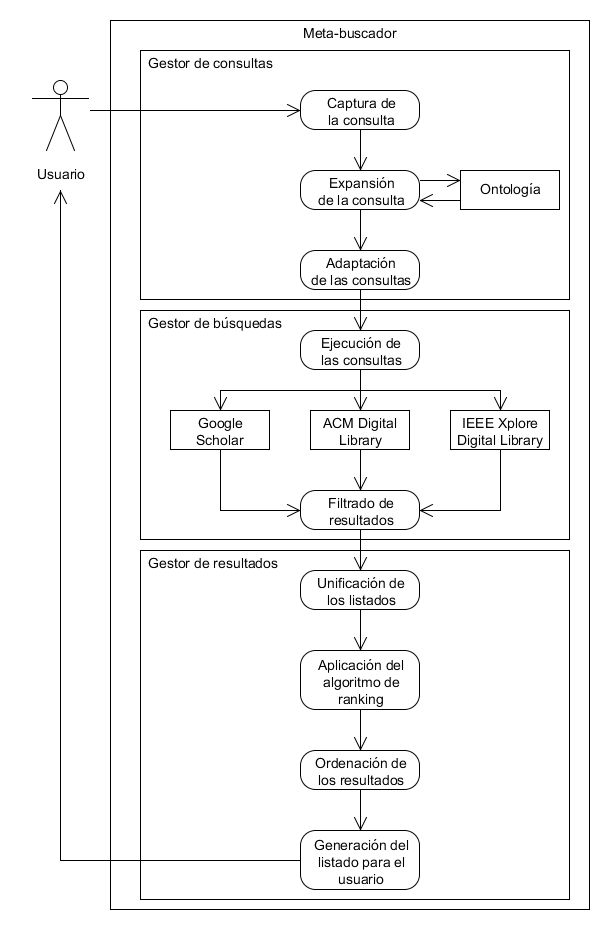
\includegraphics[width=0.4\textwidth]{img1.png}
  \label{fig:ejemplo}
\end{figure}
}

\subsection{Expansi\'on de las consultas}
\frame{
\transdissolve[duration=0.2]
\frametitle{Construcci\'on de una ontolog\'ia (I)}
El m\'etodo de expansi\'on de consultas para el meta-buscador es una ontolog\'ia. Su dise\~no requiri\'o las siguientes actividades:
\begin{itemize}
\item Definici\'on del dominio: dado el contexto de aplicaci\'on del SRI se comenz\'o por seleccionar una  sub\'area tem\'atica dentro de las Ciencias de la Computaci\'on a partir de la cual realizar la ontolog\'ia. Se determin\'o que se comenzar\'ia por la sub\'area de Inteligencia Artificial (IA).
\item Determinar los t\'erminos a incluir: se gener\'o una lista de t\'erminos a partir de una revisi\'on del estado del arte de la disciplina, obteniendo un conjunto de conceptos que caracterizan a las subdivisiones de la IA, conjuntamente se definieron sin\'onimos de cada concepto que pudieran ser utilizados en el m\'etodo de expansi\'on.
\end{itemize}
}

\frame{
\transdissolve[duration=0.2]
\frametitle{Construcci\'on de una ontolog\'ia (II)}
\begin{itemize}
\item Definici\'on de la jerarqu\'ia de clases: utilizando el m\'etodo top-down, se defini\'o como clase a todo concepto que representara una categor\'ia en la que la disciplina pudiera subdividirse, definiendo dentro de cada clase aquellas instancias que ser\'ian consideradas como subclases, con el objetivo de que la ontolog\'ia represente de la mejor manera posible la taxonom\'ia original del \'area.
\end{itemize}
}

\frame{
\transdissolve[duration=0.2]
\frametitle{Construcci\'on de una ontolog\'ia (III)}
\begin{itemize}
\item Definici\'on de propiedades de las clases: aquellos atributos que describan a los conceptos, considerando las relaciones existentes entre ellos. Se definieron relaciones impl\'icitas a partir de las conexiones entre los conceptos: 
	\begin{itemize}
	\item "Es un (padre)", simbolizando la situaci\'on de que una clase contiene a otra.
	\item "Es un (hijo)", relaci\'on inversa a la anterior, que representa que una clase es contenida por otra.
	\item "Es un (hermano)", simbolizando a un conjunto de clases que comparten un mismo "padre".
	\end{itemize}
En cuanto a relaciones expl\'icitas, aquellas definidas para dar mayor valor a la ontolog\'ia considerando su objetivo de aplicaci\'on, siendo representada por la relaci\'on de sinonimia, utilizando los t\'erminos relevados al inicio del proceso. 
\end{itemize}
}

\frame{
\transdissolve[duration=0.2]
\frametitle{Construcci\'on de una ontolog\'ia (IV)}
\begin{itemize}
\item Creaci\'on de instancias de las clases: utilizando los t\'erminos de mayor atomicidad, se definieron los conceptos que conformar\'ian las instancias de las clases de la ontolog\'ia. 
\end{itemize}
Para la implementaci\'on de este dise\~no de la ontolog\'ia se utilizo Prot\'eg\'e.
}

\frame{
\transdissolve[duration=0.2]
\frametitle{Desarrollo del m\'etodo de expansi\'on (I)}
Este m\'etodo obtendr\'a de la ontolog\'ia aquel concepto que guarde mayor similitud con la consulta ingresada por el usuario (consulta\_original) y a partir de ese concepto obtener los conceptos relacionados al mismo en forma impl\'icita y expl\'icita, padres, hermanos y sin\'onimos del t\'ermino. \\
Para esto, el algoritmo de divide en dos etapas; primero se busca el concepto de la ontolog\'ia m\'as similar a la consulta\_original (concepto\_candidato) y despu\'es se efect\'ua la expansi\'on al disponer de los conceptos relacionados.
}

\frame{
\transdissolve[duration=0.2]
\frametitle{Desarrollo del m\'etodo de expansi\'on (II)}
La b\'usqueda del concepto\_candidato consta de los siguientes pasos:
\begin{itemize}
\item Para cada t\'ermino de la consulta\_original: se recorre la ontolog\'ia en su totalidad almacenando en una colecci\'on temporal aquellos conceptos con mayor cantidad de coincidencias. 
\end{itemize}
}

\frame{
\transdissolve[duration=0.2]
\frametitle{Desarrollo del m\'etodo de expansi\'on (III)}
\begin{itemize}
\item En base al contenido de la colecci\'on resultante del paso anterior:
	\begin{itemize}
	\item Si no hay elementos: finaliza la expansi\'on sin resultados validos.
	\item Si hay un \'unico elemento: se le considera el concepto\_candidato.
	\end{itemize}
\end{itemize}
}

\frame{
\transdissolve[duration=0.2]
\frametitle{Desarrollo del m\'etodo de expansi\'on (IV)}
\begin{itemize}
\item 
	\begin{itemize}
	\item Si tiene m\'as de un elemento: se analiza cada concepto cuantificando las coincidencias sint\'acticas respecto a la consulta\_original. Si hay empate, se eval\'ua al elemento seg\'un las relaciones que tenga en la ontolog\'ia:
		\begin{itemize}
		\item Si todos tienen el mismo "padre": el concepto es el concepto\_candidato.
		\item Si no tienen el mismo "padre": se eval\'ua la cantidad de instancias contenidas por cada "padre", aquel con la mayor cantidad ser\'a el concepto\_candidato. En caso de otro empate: cada uno de los "padres" ser\'a considerado concepto\_candidato, conformando una colecci\'on nueva.
		\end{itemize}
	\end{itemize}
\end{itemize}
}

\frame{
\transdissolve[duration=0.2]
\frametitle{Desarrollo del m\'etodo de expansi\'on (V)}
Con el o los candidatos determinados, se inicia la etapa de la expansi\'on, que consta de los siguientes pasos:
\begin{itemize}
\item Se obtiene el concepto "padre" (concepto\_padre) del concepto\_candidato.
\item Se obtienen los conceptos del mismo nivel que el concepto\_candidato, dando lugar a la colecci\'on [conceptos\_hermanos].
\item Se obtienen, en caso de existir, los sin\'onimos del concepto\_candidato, dando lugar a la colecci\'on [sin\'onimos\_concepto].
\end{itemize}
}

\frame{
\transdissolve[duration=0.2]
\frametitle{Desarrollo del m\'etodo de expansi\'on (VI)}
\begin{itemize}
\item Se expande la consulta\_original haciendo uso de los elementos obtenidos a trav\'es de los pasos anteriores, las expansiones quedan conformadas seg\'un las f\'ormulas 1 a 4:
\begin{enumerate}
\item Expansi\'on\_1 = consulta\_original AND concepto\_candidato
\item Expansi\'on\_2 = concepto\_candidato AND concepto\_padre
\item Expansi\'on\_3 = concepto\_candidato OR [conceptos\_hermanos]
\item Expansi\'on\_4 = concepto\_candidato OR [sin\'onimos\_concepto]
\end{enumerate}
\end{itemize}
Al finalizar el algoritmo se cuenta con las cuatro expansiones de la consulta\_original ingresada por el usuario.
}



\subsection{Algoritmo de ranking}
\frame{
\transdissolve[duration=0.2]
\frametitle{Normalizaci\'on de las m\'etricas}
\begin{itemize}
\item Calidad de la fuente de publicaci\'on
	\begin{itemize}
	\item Revista Cient\'ifica: \'Indice SJR
		\begin{equation*}
		fuentePublicacion = \log_{10}(SJR)
		\end{equation*}
	\item Congreso Cient\'ifico: Ranking CORE
		\begin{equation*}
		fuentePublicacion = [A*:1 | A:0.75 | B:0.5 | C:0.25]
		\end{equation*}
	\end{itemize}
\item Calidad de los autores
	\begin{itemize}
	\item \'Indice H
		\begin{equation*}
		autores = \log_{10}(\sum_i\frac{indiceH_{autor_{i}}}{i})
		\end{equation*}
	\end{itemize}
\item Calidad del art\'iculo
	\begin{itemize}
	\item \'Indice AR
		\begin{equation*}
		calidadPublicacion = \log_{10}(\frac{citasRecibidas}{antig\mbox{\"u}edadPublicacion})
		\end{equation*}
	\end{itemize}
\end{itemize}
}

\frame{
\transdissolve[duration=0.2]
\frametitle{Ranking del documento}
\begin{equation*}
	ranking = \alpha(fuentePublicacion) \ + \ \beta(autores) \ + \ \gamma(calidadPublicacion)
\end{equation*}
$$\alpha,\beta,\gamma\mbox{: son factores de ajuste entre 0 y 1}$$
}


\section{DESARROLLO \& APLICACI\'ON}
\subsection{SRI: Desarrollo del prototipo}
\frame{
\transdissolve[duration=0.2]
\frametitle{}
Desarrollo del prototipo.
}

\subsection{SRI: Validaci\'on del prototipo}
\frame{
\transdissolve[duration=0.2]
\frametitle{}
Validaci\'on del prototipo.
}


\section{CONCLUSIONES}
\frame{
\transdissolve[duration=0.2]
\frametitle{}
Conlusiones finales.
}

\end{document}